\documentclass[a4paper,10pt,fleqn]{article}
\usepackage{verbatim,fancyhdr}
\usepackage[left=3cm, right=3cm, top=2.7cm, bottom=3cm]{geometry}
\usepackage{eurosym,rotating}
\usepackage[fleqn,sumlimits]{amsmath}
\usepackage{natbib}
\usepackage[final]{pdfpages}
\usepackage{arydshln}
\usepackage{multirow}
\usepackage{lineno}
\usepackage{appendix}
\usepackage{setspace}
\usepackage{xcolor,colortbl}
\pagestyle{plain}
\usepackage{bbding}
\usepackage{authblk}
\usepackage{psboxit}
\newcommand{\note}[1]{
\begin{boxitpara}{}%
\textbf{\underline{Instructions to reproduce results}} #1
\end{boxitpara}}
\newcommand{\BigComment}[1]{
\begin{boxitpara}{}%
\textbf{#1}
\end{boxitpara}}
\usepackage{setspace}
\usepackage{hyperref}
\bibpunct{(}{)}{,}{a}{,}{,}
\onehalfspacing
\usepackage{natbib,fancyhdr}
\usepackage[final]{pdfpages}
\usepackage{graphicx}
\usepackage{mathtools}
\usepackage{amssymb}
\DeclareMathOperator*{\argmax}{arg\,max}


\title{\large{Fundamentals in statistical pattern recognition - Mini project}\\ \Large{\textbf{Pen-Digit Character Recognition}}}

\author{
Group 7: Tiago Freitas Pereira, Braun Fabian, Marija Nikoli\'c}
\date{ May, 2015}

\begin{document}
\maketitle
\thispagestyle{fancy}

\section{Project description}\label{sec:description}
The objective of this project is to create a system for
recognizing hand-written digits using statistical pattern recognition techniques.
The available data was collected using a track-pad and a stylus. 
It contains the information of the trace each person did for
writing down the numbers. The points are given in drawing order.
Although the information about the point-by-point drawing order may potential improve recognition, we have decided not to use it in our project.
We reserve 3748 examples for training, 1873 examples for development and 1873 examples for testing.

As a baseline we use the neural networks (Multi-Layer Perception) with hyperbolic tangent activation function and the Mean-Square Error cost.
The network has three hidden units, whose weights are  randomly initialized (seed=0).
In the baseline the regularization parameter of 0.001 is used.
The classification error rates (CERs) for training, development and testing data set corresponding to the baseline solution are listed below:
\begin{itemize}
\item CER (train set) = 82.8175\%
\item CER (development set) = 82.5414\%
\item CER (test set) = 83.6626\%
\end{itemize}
The confusion matrix is shown in  Figure~\ref{fig:baseline}.
\begin{figure}[htbf]
  \caption{Confusion matrix (Baseline)}
  \centering 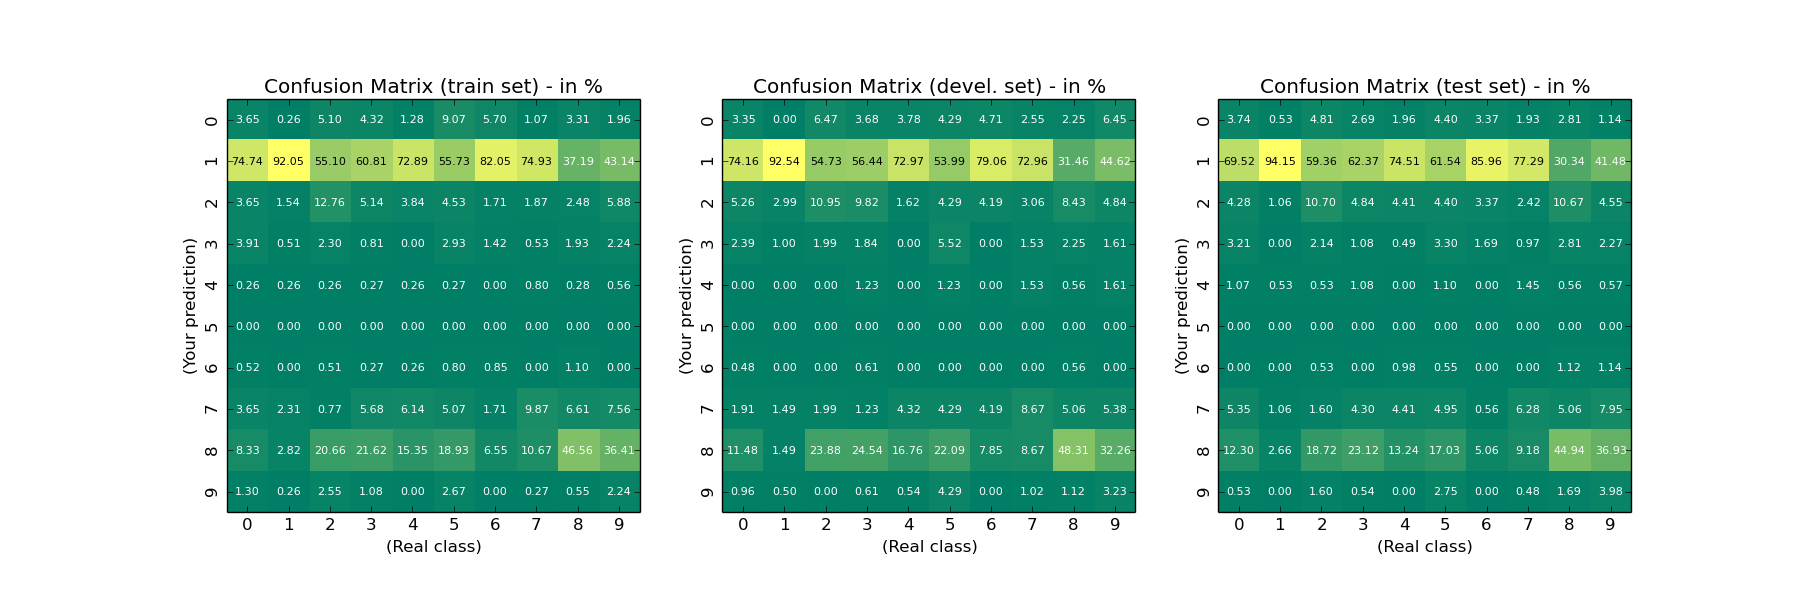
\includegraphics[width=\textwidth,height=0.3\textwidth]{Figures/baseline}
  \label{fig:baseline}
\end{figure}

In order to improve the recognition performance we have studied and implemented three different techniques.
The first technique (Section~\ref{sec:pca_mclr})  makes use of Principal Component Analysis and Multi-Class Logistic Regression (PCA-MCLR).
In the second technique  (Section~\ref{sec:pca_lda}) we employ  Linear Discriminant Analysis together with Principal Component Analysis (PCA-LDA).
The third evaluated technique  (Section~\ref{sec:pca_mlp}) refers to the Multi-Layer Perception enhanced through the use of Principal Component Analysis (PCA-MLP). 
Curse of dimensionality represents the main motivation of using Principal Component Analysis (Section~\ref{sec:pca}) in all studied techniques.

\section{Principal Component Analysis}\label{sec:pca}

The available data set consists of high-dimensional feature vectors (784 $\times$ 1) that are difficult to handle. Moreover, it is not possible to make sense of all variables and to understand the possible correlations.
Therefore, we consider data  in terms of its principal components, or equivalently, in terms of the directions where the data is most spread out. Dimension reduction is achieved by discarding the directions with the small spread.
For these purpose we consider so-called energy load curve (Figure~\ref{fig:pca}), which describes the percentage of the captured data variability with respect to the number of principal components.
Figure~\ref{fig:pca} shows that, for instance, 100, 200 and 300 principal components preserve 85.03\%, 97.89\% and 99.8\% of energy, respectively.

\begin{figure}[htbf]
  \caption{Energy load curve (PCA)}
  \centering 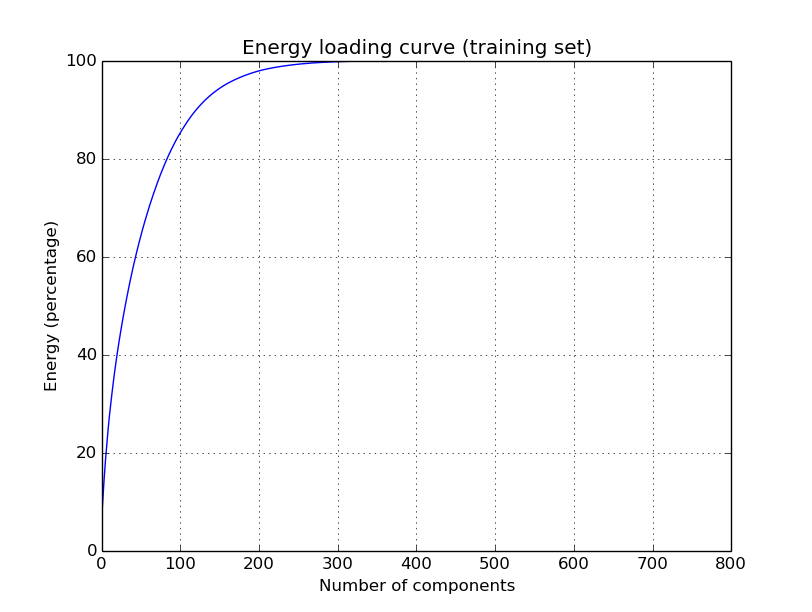
\includegraphics[width=\textwidth,height=0.7\textwidth]{Figures/energy_load_curve}
  \label{fig:pca}
\end{figure}

\section{Multi-Class Logistic Regression and Principal Component Analysis}\label{sec:pca_mclr}

We consider a multi-class classification problem where the goal is to assign an input vector X to one of K classes.
The number of classes (K) is equal to 10 (10 digits for classification) and input feature vector (X) is rearranged as 784-vector.
Here we use MCLR together with PCA (PCA-MCLR), meaning that the input vector (X) is  projected to a new space determined using PCA.

Logistic regression (LR) is a classification method with the classifier defined as

\begin{equation}\label{eq:LR}
\begin{array}{lcl}
\displaystyle class= \left\{
\begin{array}{lr}
0, & h_{\theta}(x) < 0.5\\
1, &  h_{\theta}(x) \geq 0.5,
\end{array}
\right.
\end{array}
\end{equation}
where
\begin{equation}\label{eq:h}
h_{\theta}(x) = g(\theta^T x ), \theta^T = [\theta_0 \theta_1 ... \theta_d ],
\end{equation}
with $g(x)$ being the logistic function
\begin{equation}\label{eq:g}
g(x)=\frac{1}{1 + \exp(-x)}.
\end{equation}

Logistic regression can be easily generalized to multiple classes (MCLR).
We train LR classifier $h^K_{\theta}(x)$ for each class K (K=1,...,10,) to predict the probability that class is equal to K (K vs. the rest). To make a prediction on a new input vector we choose the class such that 
\begin{equation}\label{eq:mclr}
class = \argmax_K h^K_{\theta}(x),  {K}=1,...,10.
\end{equation}

We have analyzed the performance of the PCA-MCLR using different number of principal components.
The best performance (based on the test set) is achieved using 200 principal components and the corresponding classification error rates (CERs)  are listed below:
\begin{itemize}
\item CER (train set) = 38.0203\%
\item CER (development set) = 53.2301\%
\item CER (test set) = 51.8420\%
\end{itemize}

The confusion matrix for training, development and testing data set is shown in Figure~\ref{fig:pca_mclr}.
\begin{figure}[htbf]
  \caption{Confusion matrix (PCA-MCLR)}
  \centering 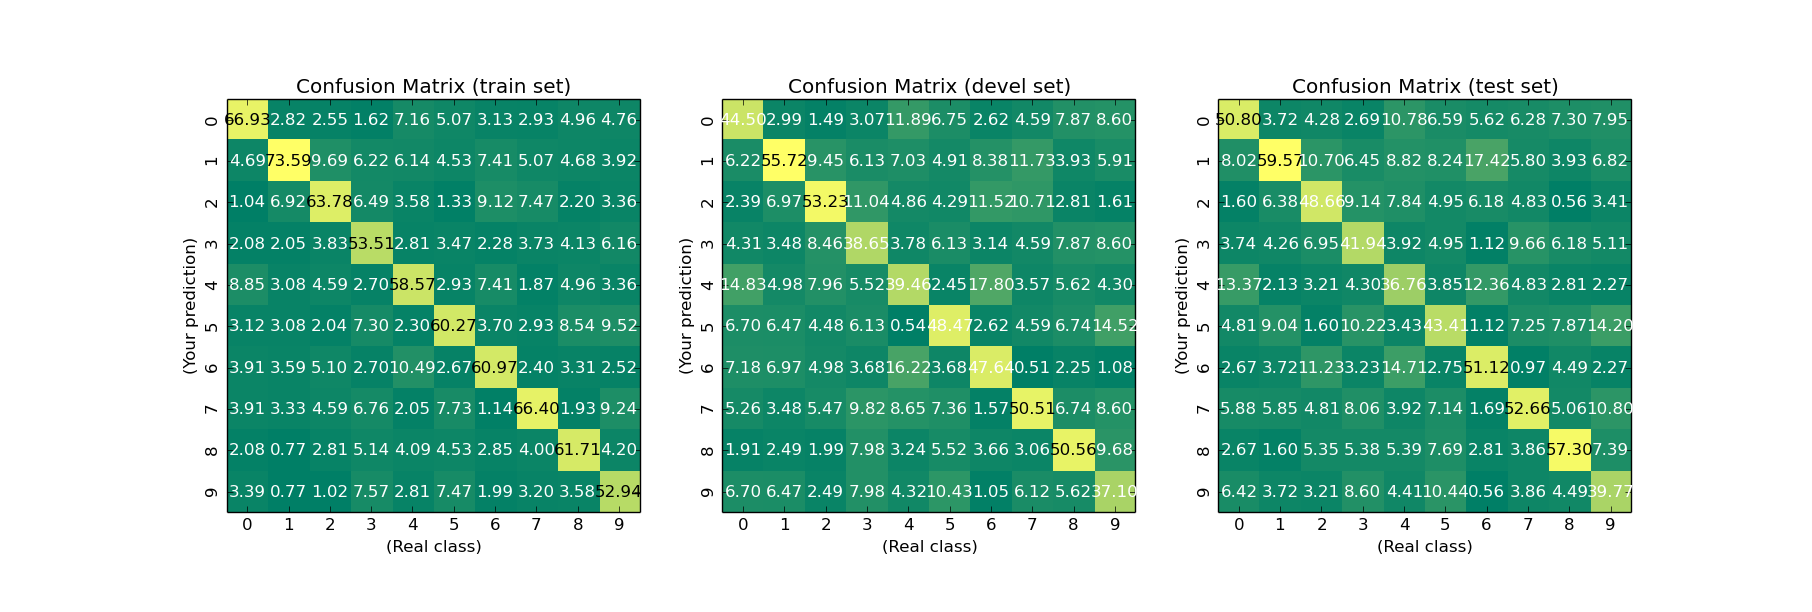
\includegraphics[width=\textwidth,height=0.3\textwidth]{Figures/mclr_pca200}
  \label{fig:pca_mclr}
\end{figure}

Note that with 200 principal directions,  97.89 \% of data variability is preserved.

Compared with the the baseline solution (Section~\ref{sec:description}), significant improvement is achieved using PCA-MCLR method.

\note{\\ \$ cd  {MiniProj\_MCLR\_PCA} \# change into directory for PCA-MCLR \\
\$ ./mclr\_train.py zero -c 200 \\
\$ ./mclr\_train.py one -c 200 \\
\$ ./mclr\_train.py two -c 200 \\
\$ ./mclr\_train.py three -c 200 \\
\$ ./mclr\_train.py four -c 200 \\
\$ ./mclr\_train.py five -c 200 \\
\$ ./mclr\_train.py six -c 200 \\
\$ ./mclr\_train.py seven -c 200 \\
\$ ./mclr\_train.py eight -c 200 \\
\$ ./mclr\_train.py nine -c 200 \\\\
\$ ./mclr\_evaluate.py zero.hdf5 one.hdf5 two.hdf5 three.hdf5 four.hdf5 five.hdf5 six.hdf5 seven.hdf5 eight.hdf5 ninie.hdf5 -c 200 -{}-test -p\\\\
\# -c: Number of principal components to keep\\
\# -{}-test: Evaluates the performance on test set\\
\# -p: Visualizes confusion matrices graphically
}

\section{Linear Discriminant Analysis and Principal Component Analysis}\label{sec:pca_lda}

The technique for recognizing hand-written digits described in this section combines LDA and PCA (PCA-LDA). As in the previous technique, PCA is used so as to achieve dimensionality reduction.
The assumption that we make for classification is that the projection of the data so that the spread is maximized, leads to  better discrimination capabilities.
In LDA, we are interested to find a subspace in which the variability is maximized between data from
different classes, and at the same time the variability in the same class is minimized. 
In a new subspace we create average models for each digit from the train data set and evaluate performance of the models on the three data sets using the cosine similarity. The cosine similarity between two vectors $p$ and $q$ is given  as
\begin{equation}\label{eq:cs}
s(p,q)=\frac{p\cdot q}{|p||q|}.
\end{equation}
We have chosen to keep the maximum possible number of LDA components (number of classes - 1 = 9).
As for the number of PCA components, different variants were tested. The best performance (based on the test set) is achieved using 200 principal components and the corresponding classification error rates (CERs)  are listed below:
\begin{itemize}
\item CER (train set) = 41.8890\%
\item CER (development set) = 54.1911\%
\item CER (test set) = 52.4826\%
\end{itemize}
The confusion matrix for training, development and testing data set is shown in Figure~\ref{fig:pca_lda}.
\begin{figure}[htbf]
  \caption{Confusion matrix (PCA-LDA)}
  \centering 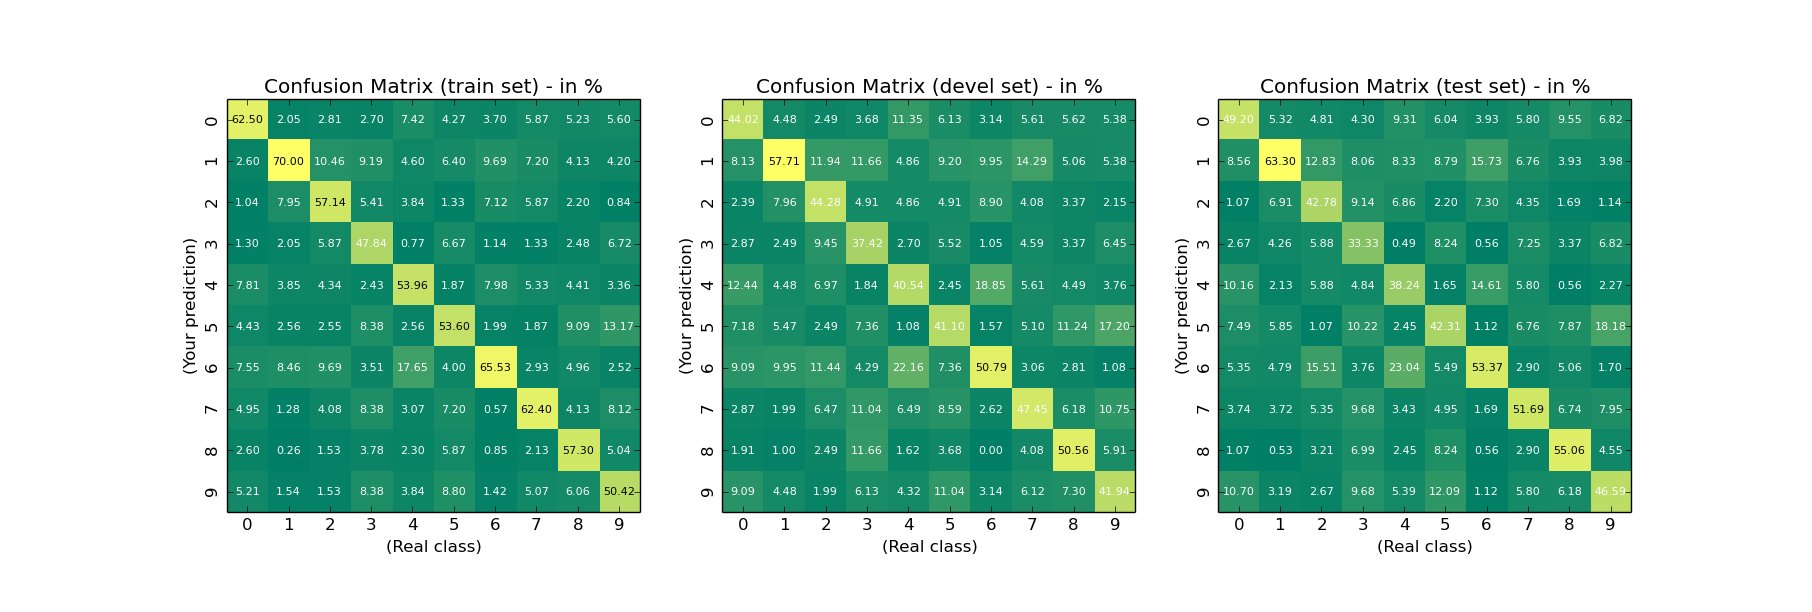
\includegraphics[width=\textwidth,height=0.3\textwidth]{Figures/pca200_lda9}
  \label{fig:pca_lda}
\end{figure}

The results presented for PCA-MCLR and PCA-LDA suggest that better recognizing performance is achieved using the former method.

\note{\\ \$ cd  {MiniProj\_PCA\_LDA} \# change into directory for PCA-LDA \\
\$ ./pca\_lda.py -c 200 -l 9 -t -p -e\\\\
\# -c: Number of principal components to keep\\
\# -l: Number of LDA components to keep\\
\# -t: Evaluates the performance on test set\\
\# -p: Visualizes confusion matrices graphically\\
\# -e: Visualizes energy load curve graphically
}
\section{ Multi-Layer Perception and Principal Component Analysis}\label{sec:pca_mlp}

\end{document}
